
% !TeX spellcheck = pt_BR
% !TEX encoding = UTF-8 Unicode

% Ver copyright.tex para direitos autorais e licença.

\clearpage
\section{Variáveis aleatórias contínuas}

\subsection{Função de densidade de probabilidade}

Considere a variável aleatória $X$ definida informalmente da seguinte maneira: "Seja $X$ um número escolhido no intervalo $(0,1)$ de forma uniforme ao acaso." Ao pensarmos com cuidado, percebemos que essa descrição é um pouco desconcertante. A palavra "uniforme" deveria significar que qualquer número $x \in (0,1)$ tem igual probabilidade de ser escolhido, ou seja, $\Pb(X = x)$ deveria ser o mesmo para cada $x$. No entanto, existem infinitos $x \in (0,1)$, o que forçaria $\Pb(X = x)$ a ser zero. Isso de fato acontecerá para todas as variáveis aleatórias com distribuições contínuas, que definimos agora.

\begin{definition}
Dizemos que uma variável aleatória $X$ é \emph{contínua, com função de densidade de probabilidade $f_X: \R \to \R$}, se
\begin{equation}
\Pb(a \leq X \leq b) = \int_{a}^{b} f_X(x) \, \dd x
\end{equation}
para todo $a < b \in \R$.
\end{definition}

Uma densidade $f_X$ especifica a "probabilidade por unidade de comprimento." É algo análogo à função de probabilidade de massa, mas não exatamente. A probabilidade de $X$ estar em um pequeno intervalo de comprimento $\Delta x$ é dada por $f_X(x) \Delta x$, em vez de $f_X(x)$, e $f_X$ em si pode assumir valores muito grandes em pequenos intervalos. Portanto, é " $f_X(x) \Delta x$ " que é análogo a $p_X(x)$.

Uma função de densidade deve satisfazer necessariamente
\[
\int_{-\infty}^{+\infty} f_X(x) \, \dd x = 1
.
\]

\subsection{Variáveis Uniformes}

Sejam $a$ e $b$ em $\R$ com $a < b$. Uma variável aleatória $X$ tem a distribuição uniforme (contínua) em $(a,b)$ se
\[
f_X(x) =
\begin{cases}
\frac{1}{b-a}&\text{se } a < x < b,\\
0&\text{caso contrário.}
\end{cases}
\]
Escrevemos $X \sim \Unif(a,b)$.\\

Observe que, para qualquer intervalo $[c,d] \subseteq [a,b]$, temos
\[
\Pb(X \in [c,d]) = \int_{c}^d \frac{1}{b-a} \, \dd x
=
\frac{d-c}{b-a}
,
\]
ou seja, o intervalo $[c,d]$ tem uma probabilidade dada pela \emph{proporção} do seu comprimento dentro do intervalo $[a,b]$. Por outro lado, se $c < a$ e $d \in [a,b]$, então
\[
\Pb(X \in [c,d])
=
\frac{d-a}{b-a}
\]
porque a parte do intervalo $[c,d]$ que não se sobrepõe com $[a,b]$ não conta.


\subsection{Distribuição Normal}

Seja $\mu \in \R$ e $\sigma > 0$. Uma variável aleatória $X$ tem distribuição normal (ou gaussiana) com parâmetros $\mu$ e $\sigma^2$ se tiver uma função de densidade de probabilidade dada por
\[
f_X(x) = \frac{1}{\sqrt{2\pi \sigma^2}} \cdot \e ^{-\frac{(x-\mu)^2}{2\sigma^2}}
\]
para todo $ x \in \R $.
Escrevemos $X \sim \Normal (\mu,\sigma^2)$.

O parâmetro $ \mu $ dá o centro da função de densidade, e o parâmetro $ \sigma^2 $ especifica a escala com que essa densidade está sendo alongada.
Através de uma mudança de variáveis na integral, podemos ver que
$X \sim \Normal (\mu,\sigma^2)$
é equivalente a
$ X = \mu + \sigma\cdot Z $ com $ Z \sim \Normal(0,1) $.
De fato, definindo $ Z = \frac{X-\mu}{\sigma} $,
\begin{align}
\Pb(a \leq Z \leq b)
&
=
\Pb(\mu + a\sigma \leq X \leq \mu+ b\sigma)
\\
&
=
\int_{\mu + a\sigma}^{\mu + a\sigma}
\frac{1}{\sqrt{2\pi \sigma^2}} \cdot \e ^{-\frac{(x-\mu)^2}{2\sigma^2}}
\, \dd x
\\
&
=
\int_a^b
\frac{1}{\sqrt{2\pi}} \cdot \e ^{-\frac{z^2}{2}}
\, \dd z
.
\end{align}

\begin{remark}
Não é fácil ver que
$ \int_{-\infty}^{+\infty} f_X(x) \, \dd x = 1 $.
Ao substituir, obtemos
\[
\int_{-\infty}^{+\infty}
\frac{1}{\sqrt{2\pi \sigma^2}} \cdot \e ^{-\frac{(x-\mu)^2}{2\sigma^2}}
\, \dd x
=
\int_{-\infty}^{+\infty}
\frac{1}{\sqrt{\pi}} \cdot \e ^{-u^2}
\, \dd u
.
\]
Portanto, é suficiente verificar que
$ \int_{-\infty}^{+\infty} e^{-x^2} = \sqrt{\pi} $.
Na maioria dos livros didáticos, isso é feito usando coordenadas polares para integrais em $ \R^2 $, mas não queremos usar esse método.
Em vez disso, usamos um truque diferente: trocamos as integrais iteradas em
\[
\int_0^{+\infty}\left(
      \int_0^{+\infty} ye^{-(1+x^2)y^2}\dd y\right)\dd x
=
\int_0^{+\infty}\left(
      \int_0^{+\infty} y e^{-x^2y^2} e^{-y^2} \dd x\right)\dd y
,
\]
o que podemos fazer porque o integrando é não-negativo.
A primeira integral pode ser calculada como
\[
\lim_{z\to{+\infty}}
\int_0^z
ye^{-(1+x^2)y^2}\dd y
=
\lim_{z\to{+\infty}}
\frac{-1}{2(1+x^2)}
\Big[
e^{-(1+x)^2 y^2}
\Big]_0^z
=
\frac{1}{2(1+x^2)}
\]
e
\[
\int_0^{+\infty}\left(
      \int_0^{+\infty} ye^{-(1+x^2)y^2}\dd y\right)\dd x
=
\lim_{z\to{+\infty}}
\int_0^{z}
\frac{1}{2(1+x^2)}
\dd x
=
\lim_{z\to{+\infty}}
\frac{\arctan z}{2}
=
\frac{\pi}{4}
.
\]
A segunda integral pode ser reescrita como
\[
\int_0^{+\infty}
\left( \int_0^{+\infty} e^{-u^2}\dd u \right)
e^{-y^2}\dd y
.
\]
Desta forma, concluímos que
$ \int_{0}^{+\infty} e^{-x^2} = \frac{\sqrt{\pi}}{2} $.
Por simetria,
$ \int_{-\infty}^{+\infty} e^{-x^2} = \sqrt{\pi} $,
que era o que queríamos.
\end{remark}

\subsection{Tempo de Vida Exponencial}

Seja $\lambda > 0$. Uma variável aleatória $X$ tem distribuição exponencial com parâmetro $\lambda$ se
\[
f_X(x) = \begin{cases} \lambda\e ^{-\lambda x} & \text{se } x > 0,
\\
0 & \text{se } x\le 0
.
\end{cases}
\]
Escrevemos $X \sim \Exp(\lambda)$.

Observe que
\[
\Pb(X>t) = e^{-\lambda t}
.
\]

A distribuição exponencial é comumente usada para modelar a vida útil de entidades que têm a propriedade de \textit{falta de memória}, normalmente objetos inanimados que não sofrem efeitos de envelhecimento.
Para explicar o que isso significa, vamos pensar nas lâmpadas. Suponhamos que a vida útil das lâmpadas de uma determinada marca tem uma distribuição Exponencial($\lambda$) (vamos assumir que ligamos a luz e não a desligamos até a lâmpada queimar). Então, a propriedade de falta de memória significa que, independentemente de a lâmpada ter sido ativada recentemente ou ter estado ativa por um certo período de tempo, a distribuição do tempo restante de vida é a mesma. Matematicamente, isso é expresso pela seguinte identidade, que vale para todos~$s,t \ge 0$:
\[\Pb(X>t+s \,|\,  X> t) = \Pb(X > s).\]

\subsection{Esperança}

\begin{definition}
[Esperança]
Seja $ X $ uma variável aleatória contínua com densidade $ f_X $.
Definimos a \emph{esperança} de $ X $, denotada por $ \E[X] $, como o número real dado por
\[
\E[X] = \int_{-\infty}^{+\infty} x \, f_X(x) \, \dd x
,
\]
desde que esta integral convirja absolutamente.
Se a integral convergir absolutamente, dizemos que $ X $ é \emph{integrável}; caso contrário, $ \E[X] $ não está definida.
\end{definition}

\begin{example}
[Uniforme]
Se $X\sim \Unif[a,b]$, então
\[
\E [X] = \int_a^b x \, \frac{1}{b-a} \, \dd x = \frac{a+b}{2}
.
\]
Isso significa que a esperança de uma variável aleatória com distribuição uniforme no intervalo $ [a,b] $ é o ponto médio do intervalo.
\end{example}

\begin{example}
[Exponencial]
Se $X\sim\Exp(\lambda)$,
então, integrando por partes,
\[
\E [X]
=
\int_0^{+\infty} x \lambda e^{-\lambda x} \, \dd x
=
\lim_{u\to{+\infty}}
\Big[
{-x}
e^{-\lambda x}
-
\tfrac{1}{\lambda}
e^{-\lambda x}
\Big]_0^u
=
\frac{1}{\lambda}
.
\qedhere
\]
\end{example}

\begin{example}
[Normal]
Suponha que $X\sim \cN (0,1)$,
Então, substituindo $ u=x^2/2 $,
\[
\int_{0}^{+\infty} x \frac{e^{-x^2/2}}{\sqrt{2\pi}}\dd x
=
\lim_{z\to{+\infty}}
\Big[
\frac{-e^{-x^2/2}}{\sqrt{2\pi}}
\Big]_0^z
=
\frac{1}{\sqrt{{2\pi}}}
.
\]
Por simetria,
\[
\int_{-\infty}^0 x \frac{e^{-x^2/2}}{\sqrt{2\pi}}\dd x
=
-\frac{1}{\sqrt{{2\pi}}}
\]
e, portanto, $ \E[X] = 0 $.
\end{example}

\begin{example}
[Cauchy]
Suponha que $ X $ é uma variável aleatória com densidade
\[
f_X(x)=
\frac{1}{\pi\cdot(1+x^2)}
.
\]
Então
\[
\int_{0}^{+\infty} x f_X(x) \, \dd x
=
\int_{0}^{+\infty} \frac{x}{\pi\cdot(1+x^2)} \dd x
\geq
\int_{1}^{+\infty} \frac{x}{\pi\cdot(1+x^2)} \dd x
,
\]
e assim
\[
\int_{0}^{+\infty} x f_X(x) \, \dd x
\geq
\int_{1}^{+\infty} \frac{1}{2 \pi x} \dd x
=
\frac{1}{2\pi}
\lim_{z\to \infty} \ln z
=
+\infty
.
\]
Neste caso, $ \E[X] $ \emph{não é definida}, apesar da simetria.
Finalmente, temos um exemplo de uma variável aleatória que \emph{não é integrável}!
\end{example}

\subsection{Variância}

\begin{proposition}
Seja $ X $ uma variável aleatória contínua com densidade $ f_X $.
Seja $ g:\R \to \R $ uma função piecewise contínua.
Então
\[
\E[g(X)] = \int_{-\infty}^{+\infty} g(x) \, f_X(x) \, \dd x
\]
se a integral convergir absolutamente, e $ \E[g(X)] $ é indefinida se não convergir absolutamente.
\end{proposition}

A analogia com a função de massa de probabilidade está resumida na Tabela~\ref{table:comparison}.

\begin{example}
[Uniforme]
Se $X\sim \Unif [a,b]$, então
\[
\E [X^2] = \int_a^b \frac{x^2}{b-a} \, \dd x = \frac{a^2+ab+b^2}{3}.
\]
\end{example}

\begin{table}[b!]
\centering
\def\arraystretch{1.7}%
\begin{tabular}{|c|c|}
\hline
$p_X$ 			&	$f_X$	\\
\hline
$p_X:\R\to\R$ 		&	$f_X:\R\to\R$	\\
$p_X(x) \geq 0$ $\forall \, x \in \R$
			& $f_X(x) \geq 0$ $\forall \, x \in \R$ \\
$\Pb(X=x)=p_X(x)$ 	& 	$\Pb(X=x)=0$ \\
$ \Pb(a \leq X \leq b) = \sum_{a \leq x \leq b} p_X(x) $
			& 	$ \Pb(a \leq X \leq b) = \int_a^b f_X(x) \dd x $ \\
$p_X(x)=\Pb(X=x)$ 	& 	definido implicitamente acima \\
$\sum_{x}p_X(x) =1$ & $\int_{-\infty}^{\infty} f_X(x) \, dx=1$ \\
$ p_X(x) \leq 1$ $\forall \, x$ & $f_X(x)$ pode ser $>1$ \\
$ \E[g(X)] = \sum_x g(x) p_X(x) $ & $ \E[g(X)] = \int_{-\infty}^{+\infty} g(x) f_X(x) \dd x $ \\
\hline
\end{tabular}
\caption{Função de massa de probabilidade e função de densidade de probabilidade.}
\label{table:comparison}
\end{table}

\begin{example}
[Exponencial]
Se $X\sim\Exp(\lambda)$,
então, integrando por partes duas vezes,
\[
\E [X^2]
=
\int_0^{+\infty} x^2 \lambda e^{-\lambda x} \, \dd x
=
\lim_{z\to{+\infty}}
\Big[
{-x^2}
e^{-\lambda x}
-
\tfrac{2x}{\lambda}
e^{-\lambda x}
-
\tfrac{2}{\lambda^2}
e^{-\lambda x}
\Big]_0^z
=
\frac{2}{\lambda^2}
.
\qedhere
\]
\end{example}

\begin{example}
[Normal]
Se $X\sim \cN (0,1)$,
então, integrando por partes,
\begin{align}
\E [X^2]
& =
\int_{-\infty}^{+\infty} x^2 \frac{e^{-x^2/2}}{\sqrt{2\pi}}\dd x
\\
&
=
2 \cdot \frac{1}{\sqrt{2\pi}}
\int_{0}^{+\infty} x \cdot (x {e^{-x^2/2}}) \, \dd x
\\
&
=
\frac{2}{\sqrt{2\pi}}
\lim_{u\to+\infty}
\Big[
{-x} {e^{-x^2/2}}
+
\int_{0}^{u}
e^{-x^2/2} \, \dd x
\Big]_0^u
\\
&
=
\frac{2}{\sqrt{2\pi}}
\int_{0}^{+\infty} {e^{-x^2/2}} \, \dd x
=
1
.
\end{align}
\end{example}

\begin{definition}
[Quadrado-integrável]
Como no caso de variáveis aleatórias discretas, dizemos que uma variável aleatória contínua é \emph{quadrado-integrável} se $ X^2 $ for integrável.
\end{definition}

Assim como no caso discreto, se uma variável aleatória for quadrado-integrável, ela será automaticamente integrável (porque $ |x| \leq 1+x^2 $).

\begin{definition}
[Variância]
Seja $ X $ uma variável aleatória contínua quadrado-integrável com densidade $ f_X $ e média $ \mu = \E[X] $.
Definimos a \emph{variância} de $ X $ como
\[
\V (X) = \E\big[ (X - \mu)^2 \big]
.
\]
\end{definition}

Como fizemos no caso de variáveis aleatórias discretas, podemos expandir a definição de variância para obter uma fórmula alternativa:
\[
\V(X) = \E[X^2] - (\E[X])^2
,
\]
que usamos nos exemplos a seguir.

\begin{example}
[Uniforme]
Se $X\sim \Unif [a,b]$, então
\[
\V(X) =
\frac{a^2+ab+b^2}{3}
-
\frac{a^2+2ab+b^2}{4}
= \frac{(b-a)^2}{12} .
\]
\end{example}

\begin{example}
[Exponencial]
Se $X\sim\Exp(\lambda)$,
então
\[ \V(X) = \frac{2}{\lambda^2} - \Big(\frac{1}{\lambda}\Big)^2 = \frac{1}{\lambda^2} .\]
\end{example}

\begin{example}
[Normal]
Se $X\sim\Normal(0,1)$,
então
\[
 \V(X) = 1 - 0^2 = 1 .
\]
\end{example}


\clearpage
\section{Uma única teoria para discretas e contínuas}

\subsection{Função de distribuição cumulativa}

Uma maneira de especificar uma distribuição de probabilidade em $ \R $ é dizer o quanto de probabilidade está à esquerda de cada ponto $ x $.
Em termos de uma variável aleatória $ X $ com a distribuição dada, essa probabilidade é uma função de $ x $.

\begin{definition}
Seja~$X$ uma variável aleatória. A \emph{função de distribuição cumulativa de~$X$} é a função~$F_X: \R \to [0,\infty)$ definida por
\[
F_X(x) = \Pb(X \le x)
\]
para todo $ x \in \R $.
\end{definition}

\subsubsection*{Outras probabilidades a partir de~$F_X$}

Agora, observamos que, embora~$F_X(x)$ seja definido como~$\Pb(X \le x)$, é possível usar~$F_X$ para obter outras probabilidades envolvendo~$X$. Fórmulas importantes são
\[\Pb(X > x) = 1 - \Pb(X \le x) = 1 - F_X(x)\]
e, para~$x < y$,
\[\Pb(x < X \le y) = \Pb(X \le y) - \Pb(X \le x) = F_X(y) - F_X(x).\]

Observe também que
\[\Pb(X = x) > 0 \quad \text{se e somente se}\quad F_X\text{ tem um salto em~$x$}\]
e, nesse caso, o tamanho do salto é a probabilidade de~$X = x$.

\subsubsection*{$F_X$ determina $ \Pb_X $}

\begin{proposition}
Se~$X$ e~$Y$ são duas variáveis aleatórias com~$F_X = F_Y$, então~$X$ e~$Y$ têm a mesma distribuição.
\end{proposition}
Essa proposição nos diz que a função de distribuição cumulativa realmente codifica a distribuição de uma variável aleatória (no sentido de que, dada a função de distribuição cumulativa, há apenas uma distribuição correspondente a ela).

Já vimos que $ F_X $ determina $ \Pb_X(\{x\}) $ para cada $ x \in \R $ e $ \Pb_X((a,b]) $ para todo $ a < b \in \R $.

Faltam-nos as ferramentas necessárias para provar que ela determina $ \Pb_X(B) $ para todo $ B \in \cB $.

\subsection{Casos discretos e contínuos}

\begin{figure}[b!]
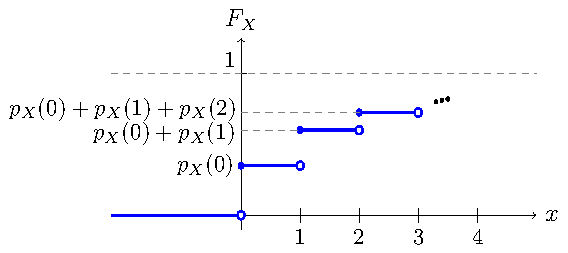
\includegraphics[width=\textwidth]{Pictures/cdfbasic}
\caption{Função de distribuição cumulativa de uma variável aleatória discreta.}
\label{fig:cdfbasic}
\end{figure}

Para obter uma primeira ideia de como se parece uma função de distribuição cumulativa, consideremos o caso em que~$X$ é discreto e tem suporte discreto contido em $\N_0$,
de modo que
\[\sum_{k=0}^\infty \Pb(X =k) = 1.\]
Em seguida, observe primeiro que
$F_X(x) = \Pb(X \le x) = 0$
para todos os $ x < 0  $.
A seguir,
e para todo $x \in [0,1)$,
\[F_X(x) = \Pb(X \le x) = \Pb(X < 0) + \Pb(X = 0) + \Pb(0 < X \le x) = 0 + p_X(0) + 0= p_X(0).\]
Ao argumentar de maneira semelhante, concluímos que
\[F_X(x) = \begin{cases} 0&\text{se } x < 0,\\ p_X(0)&\text{se } x \in [0,1),\\ p_X(0) + p_X(1)&\text{se } x \in [1,2),\\ p_X(0) + p_X(1) + p_X(2)&\text{se } x \in [2,3)\\ \cdots \end{cases}\]

O gráfico de~$F_X$ se parece com o da Figura~\ref{fig:cdfbasic}.

\begin{figure}[t]
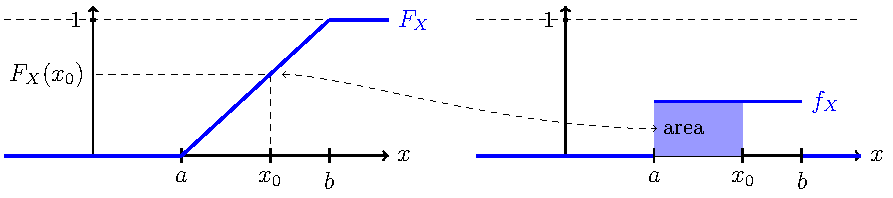
\includegraphics[width=\textwidth]{Pictures/uniform}
\caption{Função de distribuição cumulativa de uma variável aleatória uniforme.}
\label{fig:uniform}
\end{figure}

\begin{figure}[b]
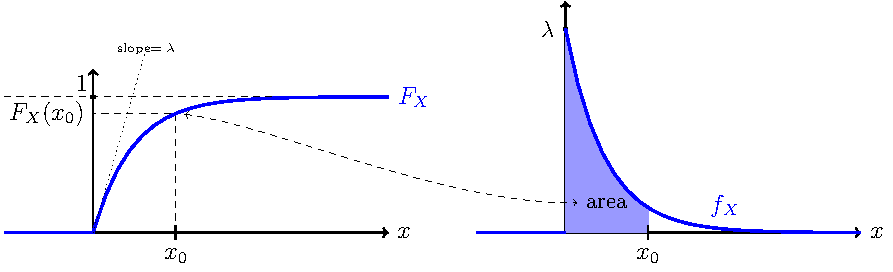
\includegraphics[width=\textwidth]{Pictures/exponential}
\caption{Função de distribuição cumulativa de uma variável aleatória exponencial.}
\label{fig:exponential}
\end{figure}

Se~$X$ for contínuo, então
\[F_X(x) = \Pb(X \le x) = \Pb(X \in (-\infty,x]) = \int_{-\infty}^x f_X(y)\dd y.\]
O teorema fundamental do Cálculo implica então que, nos pontos onde $ f_X $ é contínuo,
\[
f_X(x) = \tfrac{\dd}{\dd x} F_X'(x)
,
\]
ou seja, a função de distribuição cumulativa é diferenciável e sua derivada é a função de densidade de probabilidade.
O gráfico de~$F_X$ se parece com o das Figuras~\ref{fig:uniform} e~\ref{fig:exponential}.


\subsection{Esperança e variância}

É possível fornecer uma definição unificada de esperança de uma variável aleatória, sem assumir que ela seja discreta ou que tenha uma densidade.
Há uma fórmula mágica usando $ F_X $ que funciona simultaneamente para qualquer tipo de variável aleatória.
Não vamos nos preocupar em fornecer tal fórmula, mas é importante ter em mente que a esperança é algo que pode ser definido para qualquer variável aleatória limitada (e, desde que algumas somas ou integrais sejam convergentes, também pode ser definida para variáveis aleatórias ilimitadas).
Novamente, dizemos que $ X $ é \emph{integrável} se $ \E[X] $ for definido e finito.

Essa definição geral de esperança ainda satisfaz as três propriedades:
\begin{itemize}
\item
Unitária: $ \E[\I_A] = \Pb(A) $,
\item
Monótona:
Se $ 0 \leq Z \leq X $ para todo $ \omega\in\Omega $, então $ 0 \leq \E[Z] \leq \E[X] $,
\item
Linear: $ \E[aX+bY]=a\E[X]+b\E[Y] $
\end{itemize}
desde que $ X $ e $ Y $ sejam integráveis.

Não provaremos essas propriedades.
Claro, não poderíamos possivelmente prová-las, pois nem mesmo fornecemos a definição geral de esperança.
Mas mesmo que tivéssemos escrito a fórmula, com as ferramentas atuais não seríamos capazes de provar que a esperança é linear em geral.
A ideia da prova é a seguinte: quaisquer variáveis aleatórias $ X $ e $ Y $ podem ser aproximadas por variáveis aleatórias discretas $ X' $ e $ Y' $ e, uma vez que $ \E[X'+Y']=\E[X']+\E[Y'] $, concluímos que $ \E[X+Y]=\E[X]+\E[Y] $.

Mais uma vez, e $ X $ é \emph{quadraticamente integrável} se $ \E[X^2] $ for finito, e observe que se $ X $ é quadraticamente integrável, então ele é automaticamente integrável (porque $ |x|\leq 1+x^2 $).

\begin{definition}
[Variância]
A \emph{variância} de uma variável aleatória quadraticamente integrável $ X $ é definida como
\[
\V(X) = \E[(X-\E[X])^2]
.
\]
\end{definition}

Observamos que a desigualdade de Chebyshev é válida para qualquer variável aleatória quadraticamente integrável.
De fato, na prova dada na Seção~\ref{sub:chebyshev}, usamos apenas as propriedades de esperança mencionadas acima e nada mais.

\begin{definition}
[Covariância]
Também definimos a \emph{covariância} de duas variáveis aleatórias quadraticamente integráveis como
\[
\Cov(X,Y) = \E[(X-\E[X])(Y-\E[Y])]
\]
e dizemos que elas são \emph{não correlacionadas} se sua covariância for zero.
\end{definition}
Observe que a covariância possui todas as propriedades mencionadas na Seção~\ref{sub:covproperties}.
De fato, a prova dessas propriedades usou apenas as três propriedades de esperança mencionadas acima e nada mais.
Em particular, o Corolário~\ref{cor:uncorrelated} vale em geral, ou seja,
\[
\V(X_1+\dots+X_n)
=
\V(X_1)
+\dots+
\V(X_n)
\]
desde que $ X_1,\dots,X_n $ sejam não correlacionados.

A independência é discutida na próxima seção.

